\newpage
%==============================================={Data Collection}
\section{DATA COLLECTION}

%================================================[Coastal Zone]
\subsection{COASTAL ZONES}

To illustrate the forecasting technique on a natural time series, data is collected for coastal evolution. The study site is a 300 meter, alongshore section of south-central Wrightsville Beach, North Carolina. Figure \ref{camera_overview} illustrates the location of the camera (red star), the region of interest (yellow boundary), the camera system, and an oblique image from the dataset. The device is located on the roof of a nine-story condominium. Hourly sampling of the region began on August 22, 2013 and spans to September 1, 2015. On April 23, 2014, the beach underwent an engineered re-nourishment where sand was taken from a nearby inlet and placed on the subaerial beach and shoreface. 

In conjunction with snapshots, the camera captures a five minute video and averages frames from the video to generate a single time lapse image \cite{video_beach_monitoring}. Using an orthorectification procedure \cite{orthorectification}, image coordinates are converted to physical ground units. The oblique image of Figure \ref{camera_overview} is displayed in world coordinates in Figure \ref{classification_overview}. The image then undergoes a classification procedure using a neural network trained on RGB values of hand classified images \cite{neural_network}. The image is then post-processed to cleanly segment the image into beach, ocean, dune, and foam. More details about the camera, capturing procedure, and image segmentation can been obtained in Reference \cite{chaos_paper}.

\begin{figure}[htbp] %  figure placement: here, top, bottom, or page
   \centering
   \includegraphics[height=3in]{beach/camera_overview.pdf} 
   \caption{A: Location of Study: Wilmington, NC. B: Region of data collection. C: Solar powered camera system. D: Sample image from the camera.}
   \label{camera_overview}
\end{figure}

\begin{figure}[htbp] %  figure placement: here, top, bottom, or page
   \centering
   \includegraphics[height=3in]{beach/classification_overview.pdf} 
   \caption{(a) 3-D axes where RGB vectors from sample images are plotted and colored based on the ANN determined class (see legend). (b) A sample rectified image. (c) The image’s classified counterpart.}
   \label{classification_overview}
\end{figure}

After segmentation, the width of the beach is calculated. The profile of the inter-tidal region is constructed by plotting the beach width against the tidal level having corrected for swash run-up and setup due to gradients in breaking wave heights \cite{intertidal_esitimation}. The daily intertidal profile is then interpolated to give continuous values at all tidal levels. Finally, the daily profiles are concatenated over the study period (Figure \ref{beach}). 

The study period is split into pre-nourishment and post-nourishment segments. The pre-nourishment data spans from August 22, 2013 to April 23, 2014. The post-nourishment data spans from April 24, 2014 to September 1, 2015.


\begin{figure}[htbp] %  figure placement: here, top, bottom, or page
   \centering
   \includegraphics[width=5in]{beach/raw_beach.pdf} 
   \caption{Intertidal profile height plotted against time. Top panel is pre-nourishment. Bottom panel is post-nourishment.}
   \label{beach}
\end{figure}





%================================================[Coral Zone]
\subsection{CORAL REEFS}

For an additional illustration of nonlinear forecasting on natural data, photographic data of coral reefs are collected. Specifically, images of the benthos were captured along islands within the Line Islands Chain in the Equatorial Pacific by a team from the Scripps Institution of Oceanography (SIO). Divers swam over coral reefs in organized patterns and used specialized underwater cameras to capture a series of overlapping images. A team at the University of Miami stitched together images captured from the divers to create a single large mosaic image of the reef (Figure \ref{coral_mosaic}). Marine biology graduate students at SIO then manually scanned the mosaic images to identify each benthic species within the image. Figure \ref{classified_mosaic} shows a manually classified image, where each color represents a different species.

\begin{figure}[htbp] %  figure placement: here, top, bottom, or page
   \centering
   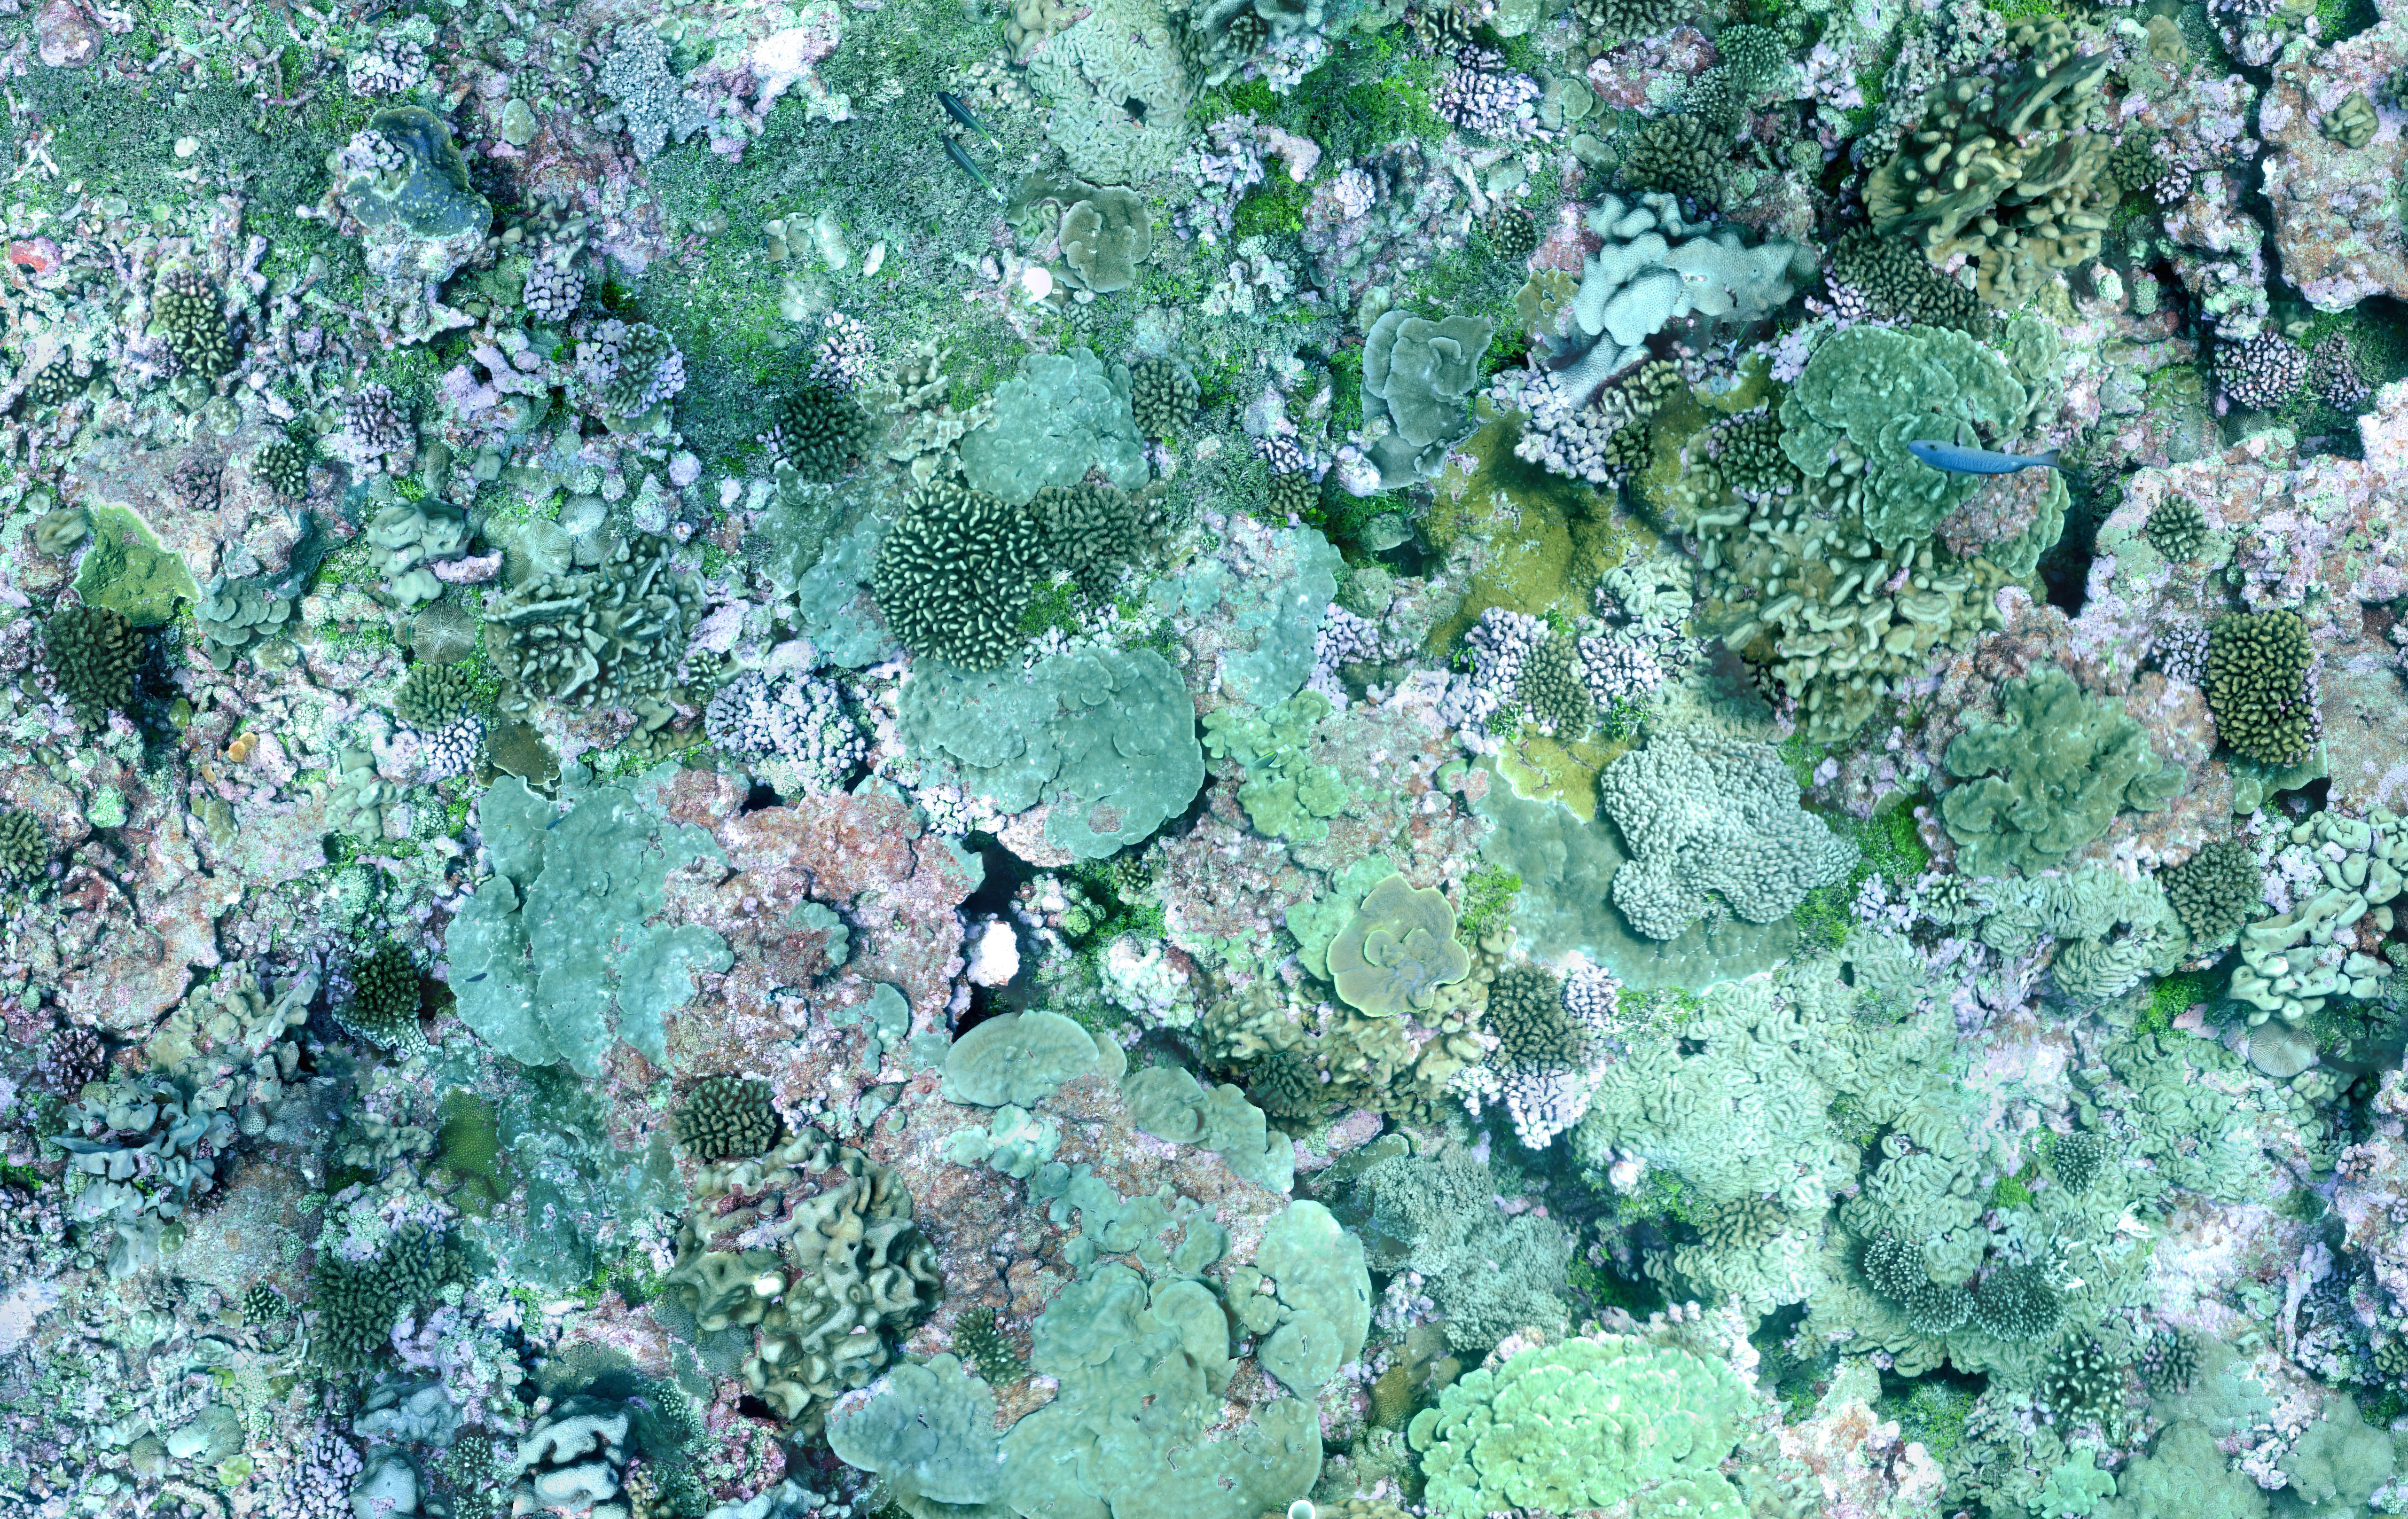
\includegraphics[width=5in]{coral/FR3_raw.jpg} 
   \caption{A portion of the raw photo-mosaic from Palmyra Island.}
   \label{coral_mosaic}
\end{figure}

\begin{figure}[htbp] %  figure placement: here, top, bottom, or page
   \centering
   \includegraphics[width=5in]{coral/FR3_class.jpg} 
   \caption{A portion of a classified photo-mosaic from Palmyra Island. Each color corresponds to a different coral or algae benthic species.}
   \label{classified_mosaic}
\end{figure}


Mosaics were collected in 2012 and again in 2013 at three islands within the Line Islands (Palmyra, Fanning, and Christmas). At each island, 20 meter by 20 meter zones were identified for monitoring and given a unique name for efficient data collection. Each island contains different human influence on coral reef habitat as the populations, water pollution, and sediment concentrations in the water vary between islands.  These varying degrees of human activity have caused correspondingly different levels of coral health \cite{line_islands_gradient} (Table \ref{coral_data}).  Manually classified mosaics for each of the islands studied here are shown in Figure \ref{coral_zones} where species have been coalesced into different morphological groupings.



\begin{table}[htbp]
\caption{Coral Zone Summary}
\begin{center}
\begin{tabular}{| l || c | c | c | c|}
  \hline       
  Zone & Location & Population & Coral Health & Study Sites\\
  \hline
  Palmyra & $5.8833^\circ$N, $162.0833^\circ$ W & 4 & Great & FR 3, 5, 7, 9 \\
  Fanning & $3.825^\circ$N, $162.349S^\circ$W & 2,500 & Good & FB 3, 4, 6, 9, 10, 11  \\
  Christmas &  $2.008^\circ$N, $157.489^\circ$W & 5,000 & Poor & KB4 \\
  \hline  
\end{tabular}
\end{center}
\label{coral_data}
\end{table}



\begin{figure}[htbp] %  figure placement: here, top, bottom, or page
   \centering
   \includegraphics[width=6in]{coral/coral_zones_all.pdf} 
   \caption{Manually classified photo-mosaics from Palmyra, Fanning, and Christmas islands. Each color corresponds to a different benthic morphological group. Image size is 1,500x1,500 pixels.}
   \label{coral_zones}
\end{figure}

















%
